Transaction throughput is a key benchmark for the performance of transactional
databases. Systems with stronger isolation levels tend to have lower transaction
throughout resulting from the increased number of aborted transactions.
Therefore, in this experiment, transaction throughput is used to determine the
performance impact of serializability in NVRAM-based key-value stores.

\subsubsection{Setup}

In order to perform this experiment, one not only needs data to work on but also
a set of concrete transactions and the operations they are composed of, i.e. a
workload. As with data, it is hard to acquire actual transaction traces and
determine their relevance. For that reason, the experiment setup relies heavily
on randomly generated data. However, each random choice is reproducible as the
generated data are stored on disk prior to the experiment. Hence, the only
non-deterministic behaviour is induced by multi-threading, the operating system,
and the underlying hardware.

\paragraph{Data}

For uniformity, this experiment uses the exact same sets of random key-value
pairs that are used in Chapter \ref{ch:eval-baseline}. Thus, there is one data
set with 1K entries and another with 100K entries. When the experiment starts,
each individual KVS will be populated with these key-value pairs.

\paragraph{Workloads}

All transactions that are to be executed during the experiment are encoded as a
workload. A workload specifies for each transaction its operations and the
respective key-value pairs to operate on. When generating a workload, there are
three important dimensions:

\begin{itemize}
    \item length of transactions
    \item number of transactions
    \item relative distribution of operations
\end{itemize}

The length of a transaction is the number of operations enclosed in that
transaction. Intuitively, the length of transactions should vary. Unfortunately,
no reliable sources as to the absolute quantities of transaction lengths could
be found. As a result, the following ranges are deemed meaningful:

\begin{figure}[!h]
    \centering
    \begin{tabular}{|l|l|l|}
        \hline
        \textbf{Name} & \textbf{Min. No. Ops} & \textbf{Max. No. Ops} \\
        \hline
        Short         & 2  & 32  \\
        Long          & 64 & 256 \\
        \hline
    \end{tabular}
    \caption{Types of transactions in terms of length.}
    \label{tab:tx-length}
\end{figure}

Short transactions can be small updates like incrementing a numeric value,
optionally based a small aggregation. Long transaction on the other hand, can be
larger aggregations such as computing a sum over many items.

When specifying the operations of a transaction, it must be decided whether an
operation reads or updates an item. Insert and delete operations are omitted as
they complicate the experiment when run concurrently. For example, a concurrent
transaction might fail because an expected pair has not been inserted yet. Such
an incident reduces transaction throughput without an actual conflict which
could distort results. The remaining two operations are selected based on the
empirical analysis in \cite{andrei2017sap}. According to the source, read
operations amount of 84\% of all operations. The remaining 16\% are sumsumed as
updates for this experiment. Each operation acts on keys from the dummy set that
are selected randomly during the workload generation. All pseudo-random numbers
were generated using uniform distributions based on seperate mersenne twister
engines. Each workload consists of 1000 transactions.

\paragraph{Scenarios}

Resulting from the dimensions shown above, four unique scenarios  were derived:

\begin{enumerate}
    \item small database, short transactions
    \item small database, long transactions
    \item large database, short transactions
    \item large database, long transactions
\end{enumerate}

These scenarios are supposed to simulate both low and high contention in
different forms. In a database that is small compared to the number of
concurrent transactions, it is very likely that multiple transactions operate on
the same data which can cause conflicts. Likewise, longer transactions cause
contention as they are more likely to access data of other transactions. That
said, scenario 1 and especially scenario 2 simulate high contention which is the
worst-case for any concurrency control. The reason is that contention often
causes conflicts which lead to aborts and reduced transaction throughput. With
larger databases, short transactions are less likely to access the same data
which reduces contention. However, as transactions become longer, they become
more likely to collide and abort.

\subsubsection{Procedure}

\begin{enumerate}
    \item populate store with dummy data (use same data from baseline benchmark)
    \item load 1 out of 4 pre-generated workloads (set of 1000 transactions with varying length working on varying data)
    \item distribute workload on pre-defined number of cores (1000 / num\_threads + amortization of remainder)
    \item fork threads with partial workloads
    \item each thread runs its transactions on the dummy data (repeats up to 3 times on failure, does not count tx if 4 attempts failed)
    \item measure time between fork and join (because timers on different cores are not synchronous)
    \item determine transaction throughput = num\_committed\_transactions / total\_time
    \item repeat this process 10 times for each workload (each workload is tied to a certain database size)
    \item after ten times: compute tx throughput, throughput speed up, parallel efficiency, and abort rate
\end{enumerate}

\subsubsection{Results}

\todo[inline]{The plots are already there (see below)}

\begin{figure}
\begin{minipage}[l]{0.50\textwidth}
        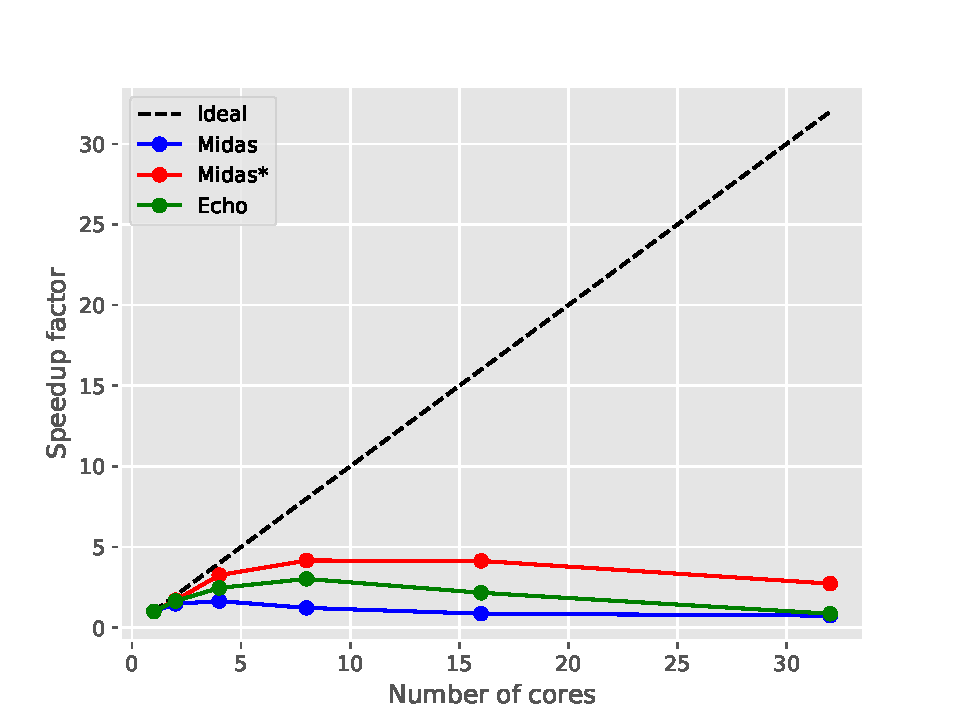
\includegraphics[width=\textwidth]{figures/bench/spd-ss}
        \caption{Transaction throughput speedup for scenario A}
        % \label{fig:concept-two-level-store}
\end{minipage}
\begin{minipage}[l]{0.50\textwidth}
    % \begin{figure}
        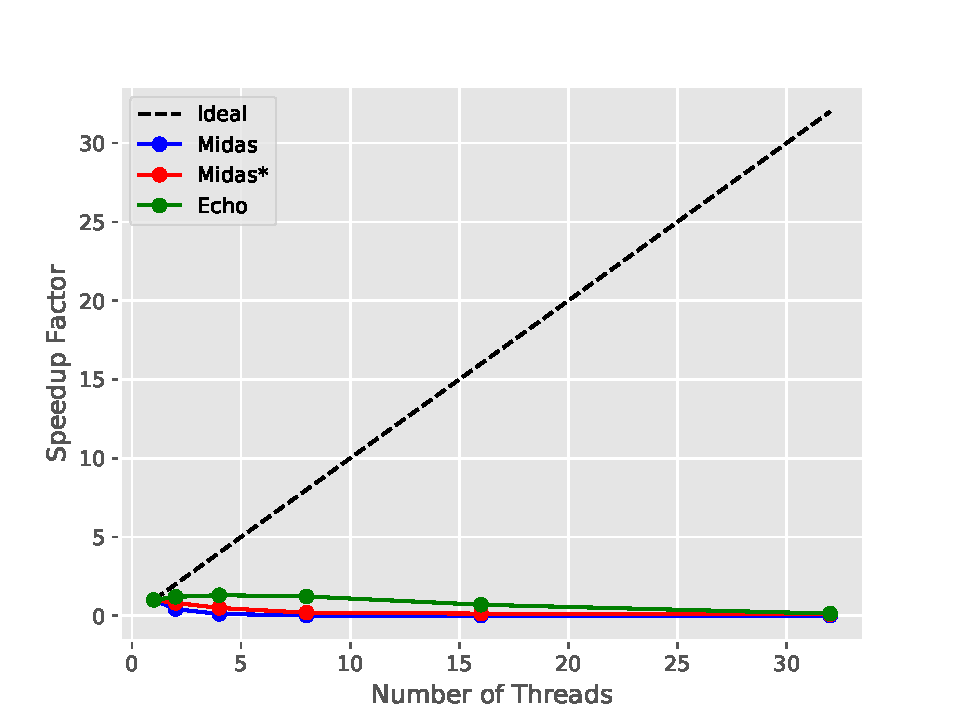
\includegraphics[width=\textwidth]{figures/bench/spd-sl}
        \caption{Transaction throughput speedup for scenario B}
        % \label{fig:concept-two-level-store}
    % \end{figure}
\end{minipage}
% \end{figure}

% \begin{figure}
\begin{minipage}[l]{0.50\textwidth}
        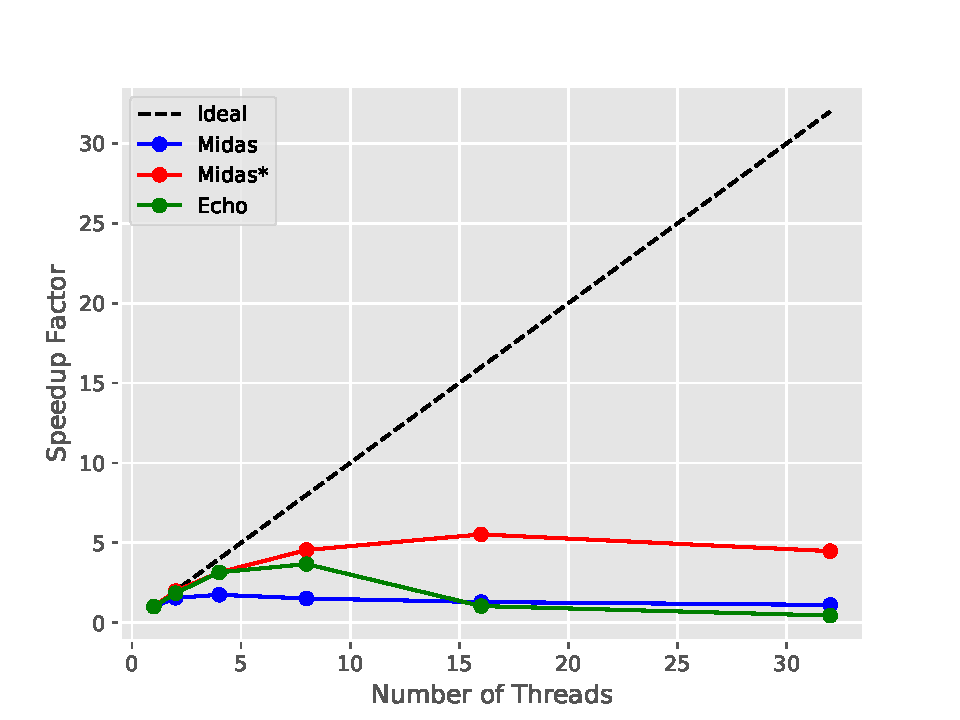
\includegraphics[width=\textwidth]{figures/bench/spd-ls}
        \caption{Transaction throughput speedup for scenario C}
        % \label{fig:concept-two-level-store}
    % \end{figure}
\end{minipage}
\begin{minipage}[l]{0.50\textwidth}
    % \begin{figure}
        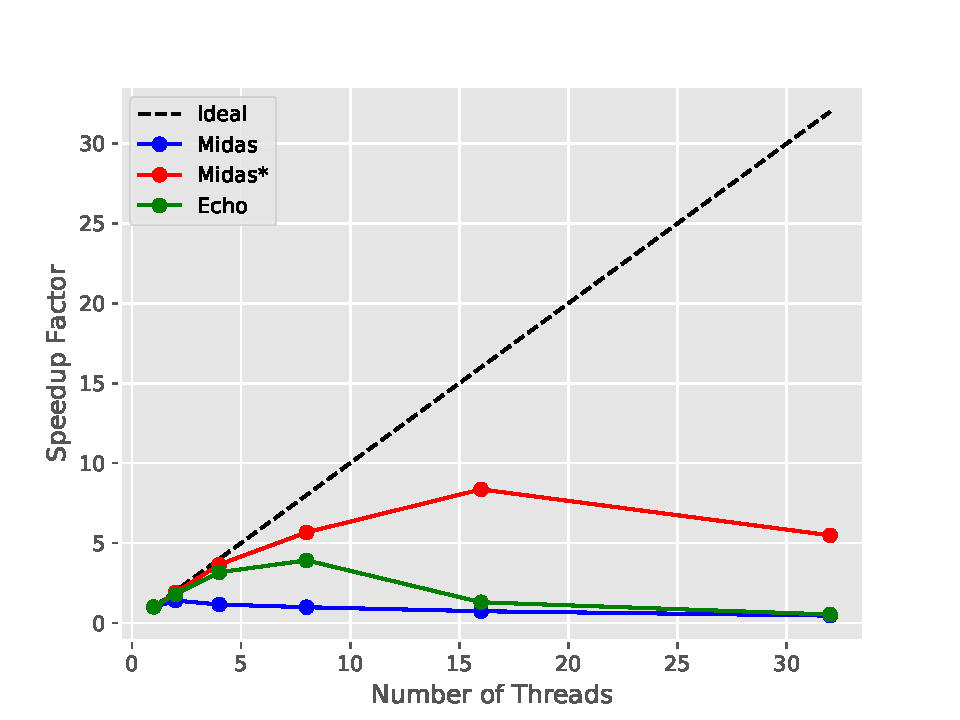
\includegraphics[width=\textwidth]{figures/bench/spd-ll}
        \caption{Transaction throughput speedup for scenario D}
        % \label{fig:concept-two-level-store}
\end{minipage}
\end{figure}

%==============================================================================
%==============================================================================
%==============================================================================

\begin{figure}
\begin{minipage}[l]{0.50\textwidth}
        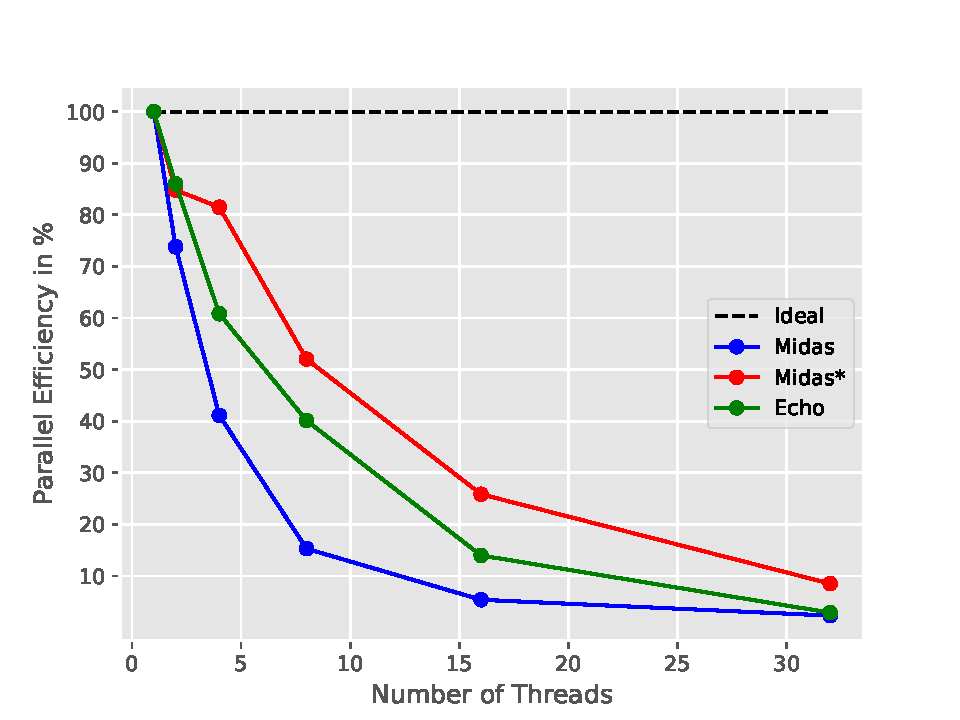
\includegraphics[width=\textwidth]{figures/bench/eff-ss}
        \caption{Parallel efficiency for scenario A}
        % \label{fig:concept-two-level-store}
\end{minipage}
\begin{minipage}[l]{0.50\textwidth}
    % \begin{figure}
        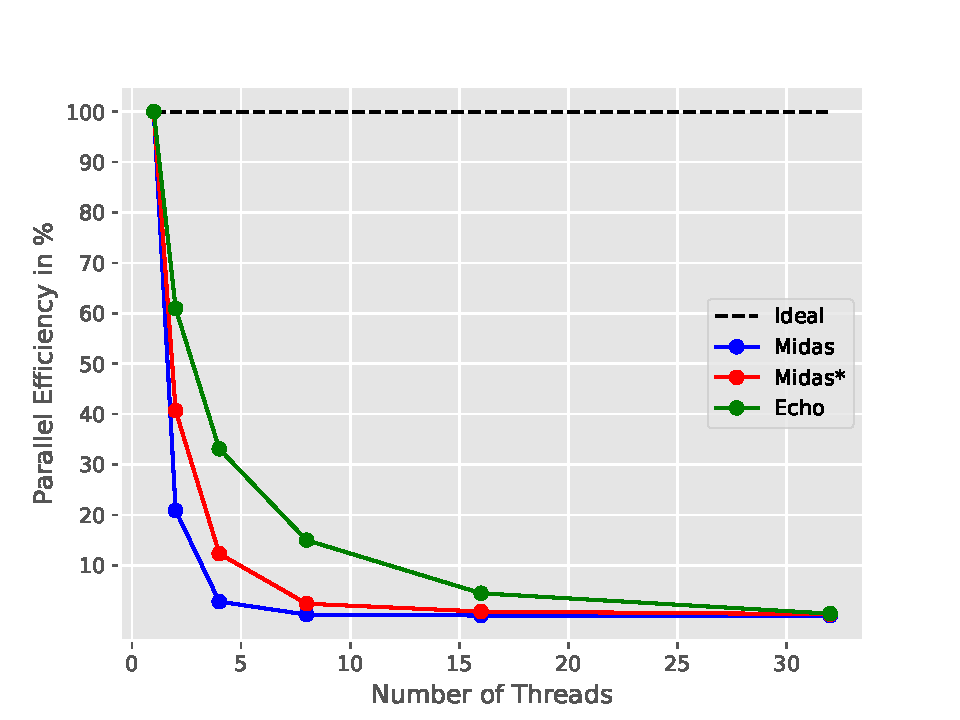
\includegraphics[width=\textwidth]{figures/bench/eff-sl}
        \caption{Parallel efficiency for scenario B}
        % \label{fig:concept-two-level-store}
    % \end{figure}
\end{minipage}
% \end{figure}

% \begin{figure}
\begin{minipage}[l]{0.50\textwidth}
        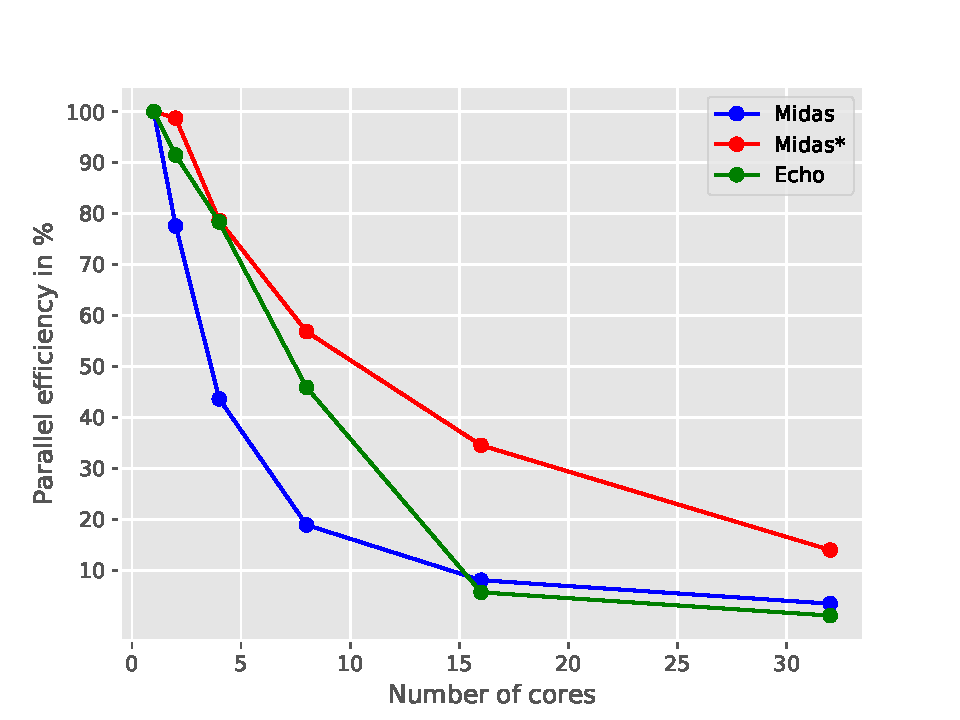
\includegraphics[width=\textwidth]{figures/bench/eff-ls}
        \caption{Parallel efficiency for scenario C}
        % \label{fig:concept-two-level-store}
    % \end{figure}
\end{minipage}
\begin{minipage}[l]{0.50\textwidth}
    % \begin{figure}
        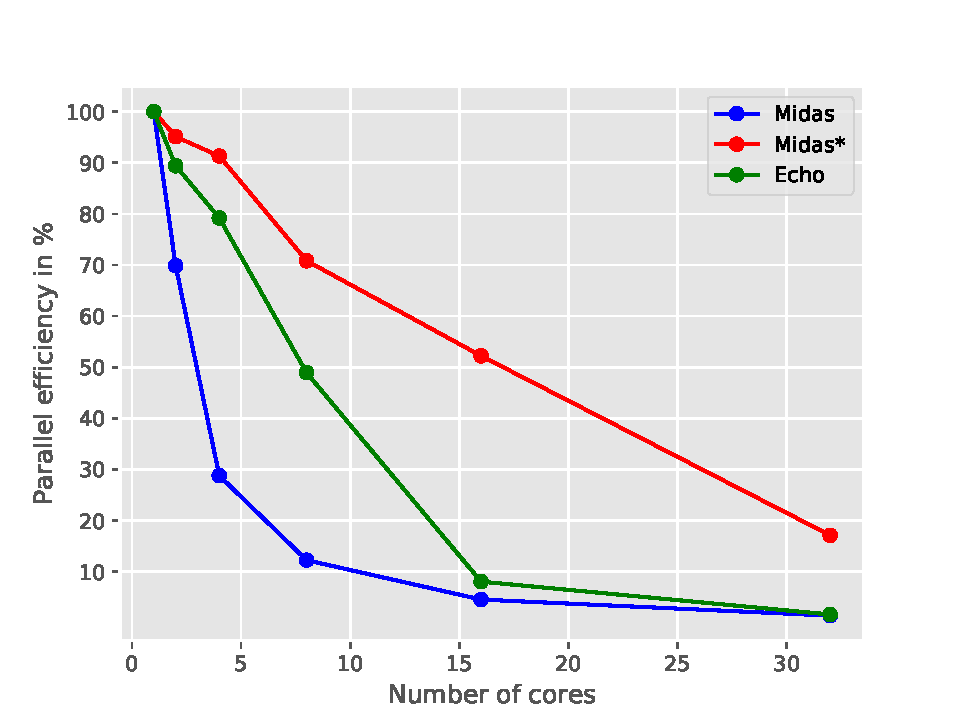
\includegraphics[width=\textwidth]{figures/bench/eff-ll}
        \caption{Parallel efficiency for scenario D}
        % \label{fig:concept-two-level-store}
\end{minipage}
\end{figure}

%==============================================================================
%==============================================================================
%==============================================================================

\begin{figure}
\begin{minipage}[l]{0.50\textwidth}
        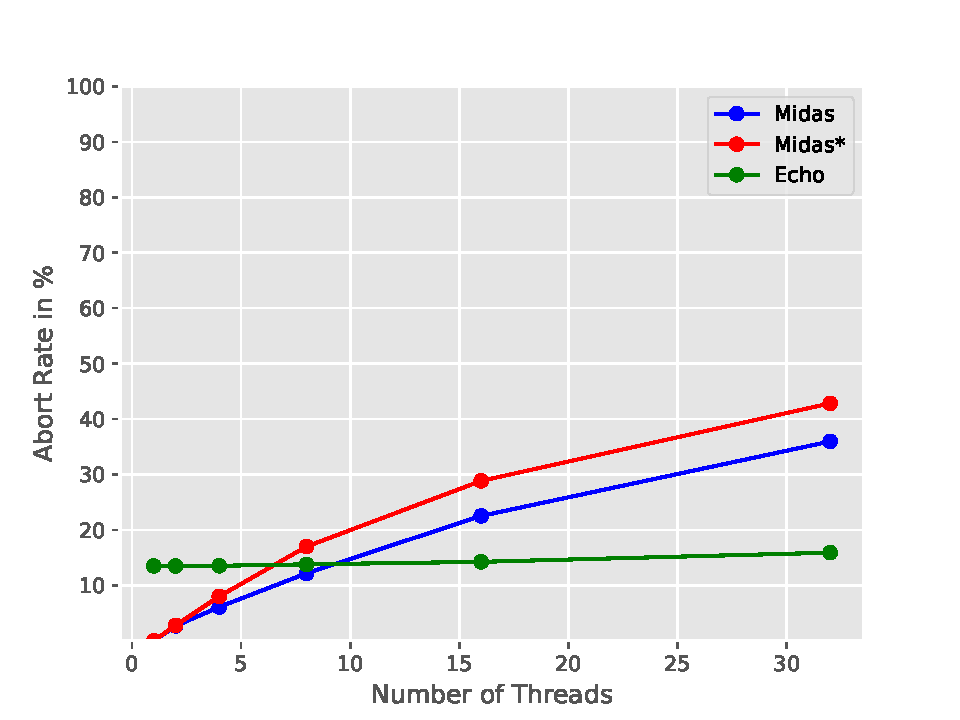
\includegraphics[width=\textwidth]{figures/bench/ar-ss}
        \caption{Abort rates for scenario A}
        % \label{fig:concept-two-level-store}
\end{minipage}
\begin{minipage}[l]{0.50\textwidth}
    % \begin{figure}
        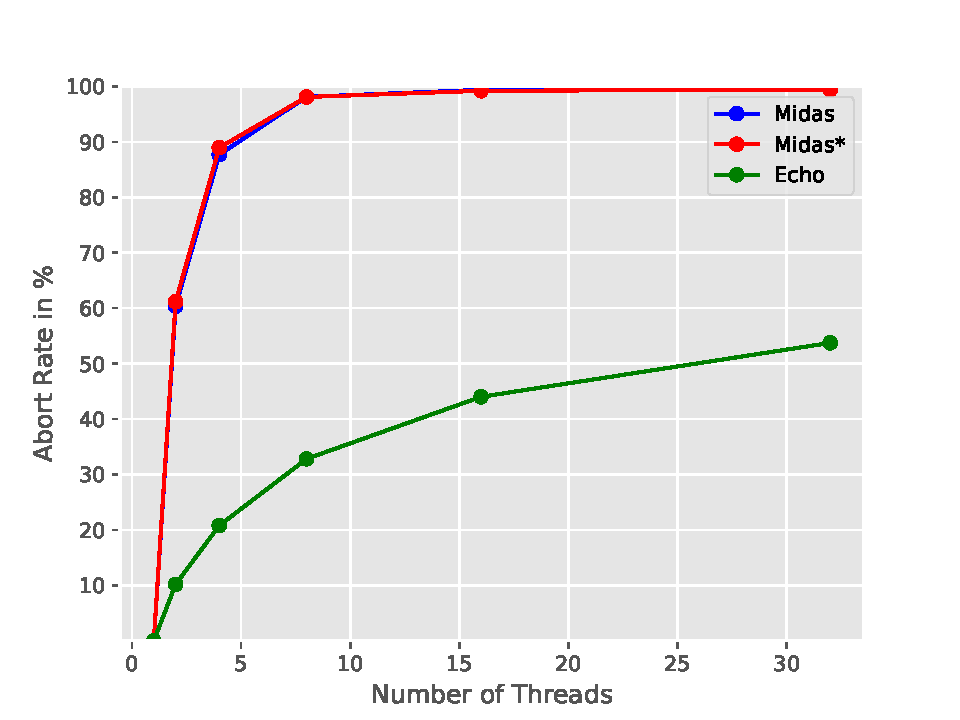
\includegraphics[width=\textwidth]{figures/bench/ar-sl}
        \caption{Abort rates for scenario B}
        % \label{fig:concept-two-level-store}
    % \end{figure}
\end{minipage}
% \end{figure}

% \begin{figure}
\begin{minipage}[l]{0.50\textwidth}
        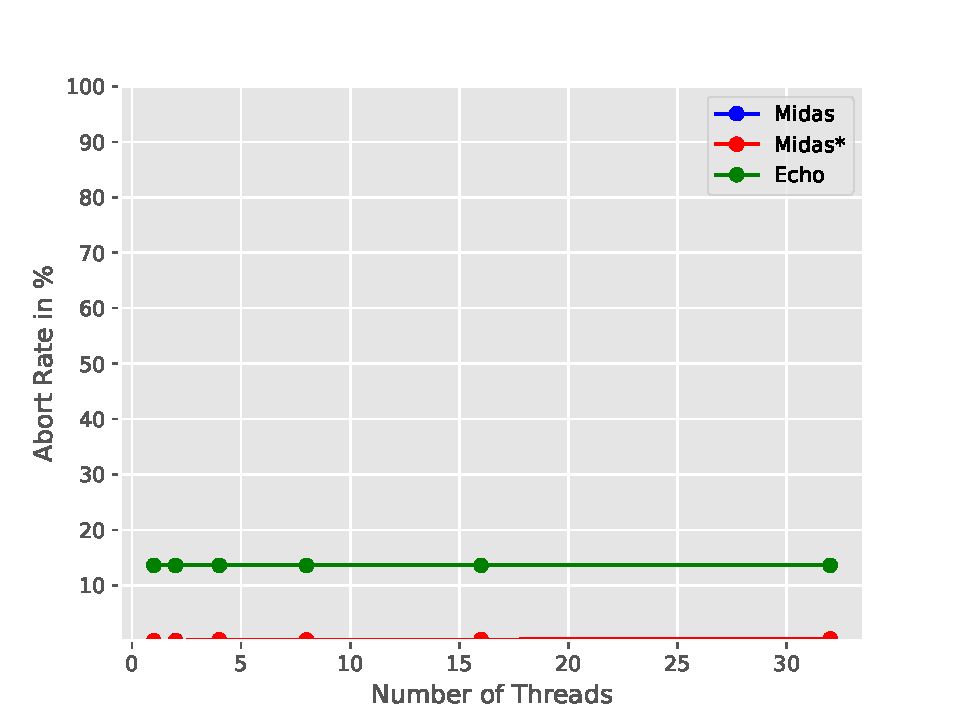
\includegraphics[width=\textwidth]{figures/bench/ar-ls}
        \caption{Abort rates for scenario C}
        % \label{fig:concept-two-level-store}
    % \end{figure}
\end{minipage}
\begin{minipage}[l]{0.50\textwidth}
    % \begin{figure}
        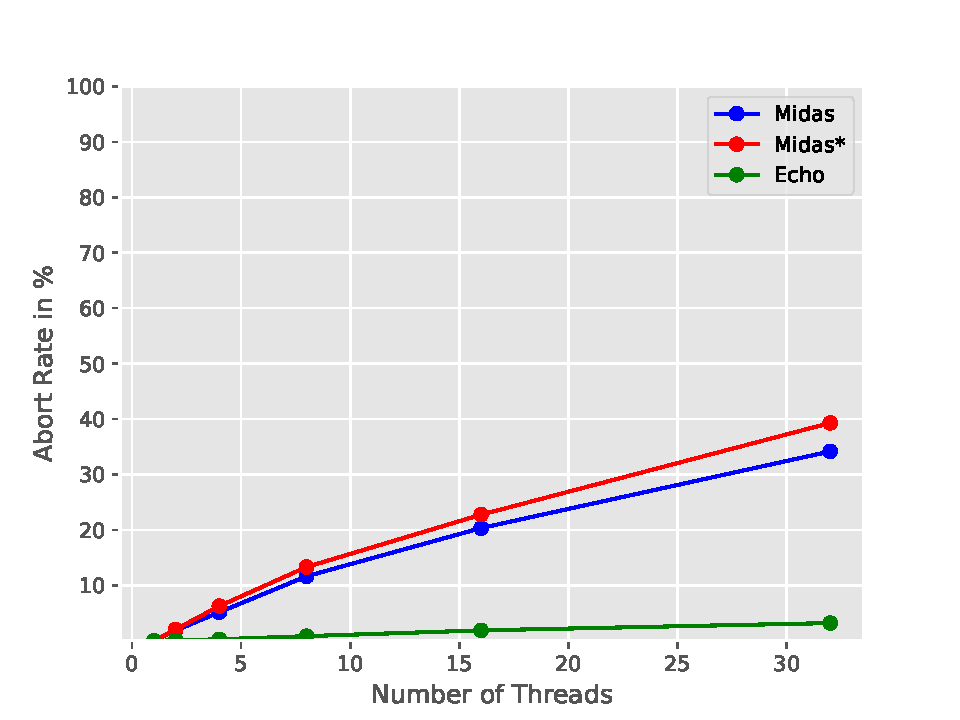
\includegraphics[width=\textwidth]{figures/bench/ar-ll}
        \caption{Abort rates for scenario D}
        % \label{fig:concept-two-level-store}
\end{minipage}
\end{figure}

\subsubsection{Discussion}

\todo[inline]{discuss results}
